The input layer is a layer that allows users of the harp to interact with the hardware itself so it may play noises or change the corresponding noises that may play while displaying a visual on the touch screen

\subsection{Laser Diodes Subsystem}
The laser Diode subsystem is a hardware component in which the user can interact with the lasers, when the lasers are interacted with the software will decide what laser has been interacted with and create a noise through the sound multiplexer


\begin{figure}[h!]
	\centering
 	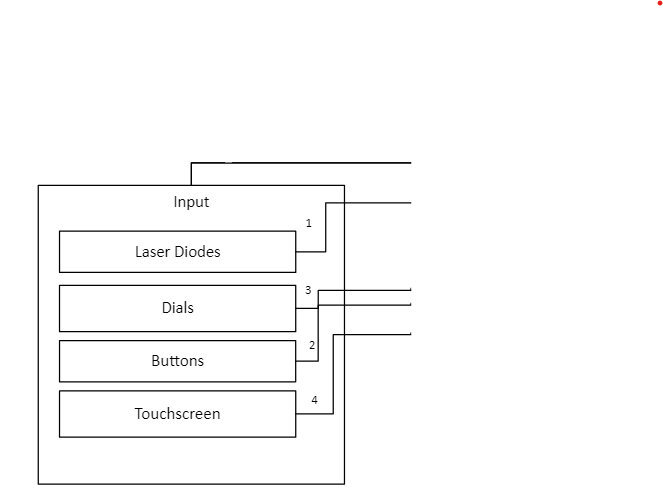
\includegraphics[width=0.60\textwidth]{images/InputSubsystem}
 \caption{Laser Diodes Subsystem}
\end{figure}

\subsubsection{Assumptions}
It is assumed that the laser system will be used in a proper way by breaking the contact of the laser diode and photo transistor

\subsubsection{Responsibilities}
Interacted by the user in order to interact with the control unit subsection in order to make noise


\subsubsection{Subsystem Interfaces}

\begin {table}[H]
\caption {Subsystem interfaces} 
\begin{center}
    \begin{tabular}{|  p{1cm}  |p{6cm}  |p{3cm}  |p{3cm} |}
    \hline
    ID & Description & Inputs & Outputs \\ \hline
    \#1& Powers a Laser Diode wich can be interacted with& User Input& \pbox{3cm}{Sound Multiplexer}\\\hline
    \end{tabular}
\end{center}
\end{table}




\subsection{Dials Subsystem}
The Dials are a subsystem which interacts with the Control unit in order to change octaves are instruments which can be selected


\begin{figure}[h!]
	\centering
 	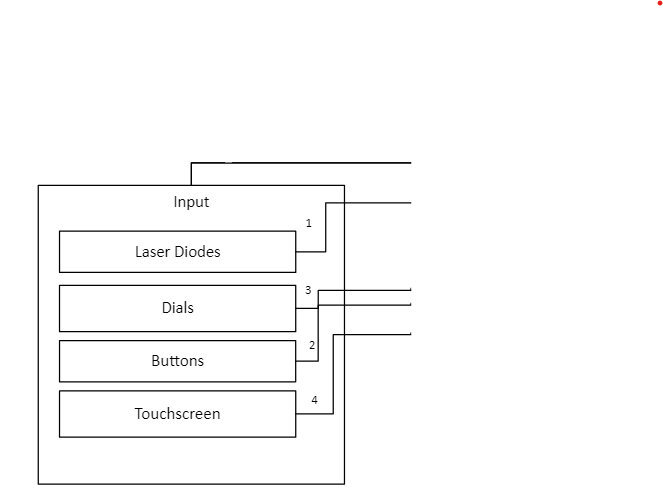
\includegraphics[width=0.60\textwidth]{images/InputSubsystem}
 \caption{Dials}
\end{figure}

\subsubsection{Assumptions}
 Dials should be rotated in a horizontal movement in order for the system to register input


\subsubsection{Responsibilities}
Dials will be used to control the sound setting which can be used to turn up or turn down the sound of the harp through the speakers

\subsubsection{Subsystem Interfaces}

\begin {table}[H]
\caption {Subsystem interfaces} 
\begin{center}
    \begin{tabular}{|  p{1cm}  |p{6cm}  |p{3cm}  |p{3cm} |}
    \hline
    ID & Description & Inputs & Outputs \\ \hline
    \#1& Used to adjust the sound setting & Human input& \pbox{3cm}{Speaker}\\\hline
    \end{tabular}
\end{center}
\end{table}



\subsection{Buttons Subsystem}
Buttons are used to change octaves or interact with different areas of the control unit.

\begin{figure}[h!]
	\centering
 	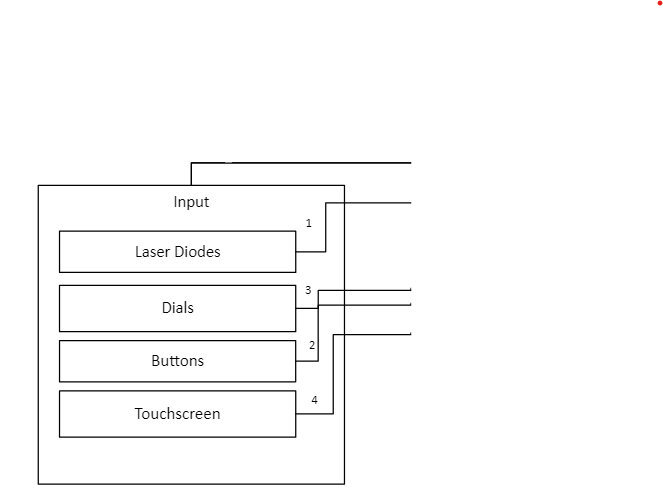
\includegraphics[width=0.60\textwidth]{images/InputSubsystem}
 \caption{Buttons}
\end{figure}

\subsubsection{Assumptions}
A assumption to be made for the buttons is that they are used as a alternative way as a input for the control unit


\subsubsection{Responsibilities}
The responsibility of the button is to control the sound settings and interact with the sound settings such as lowering the volume and the user settings such as changing octave or instruments 


\subsubsection{Subsystem Interfaces}

\begin {table}[H]
\caption {Subsystem interfaces} 
\begin{center}
    \begin{tabular}{|  p{1cm}  |p{6cm}  |p{3cm}  |p{4cm}|}
    \hline
    ID & Description & Inputs & Outputs \\ \hline
    \#1& Round buttons which may be pressed in order to change sound levels or instruments& User input&       Sound Settings and user Settings\\\hline
    \end{tabular}
\end{center}
\end{table}

\subsection{Touchscreen Subsystem}
The touchscreen is used for visual display and to display certain elements of settings to the user, the touchscreen can be used as a alternative way to interact with the control unit


\begin{figure}[h!]
	\centering
 	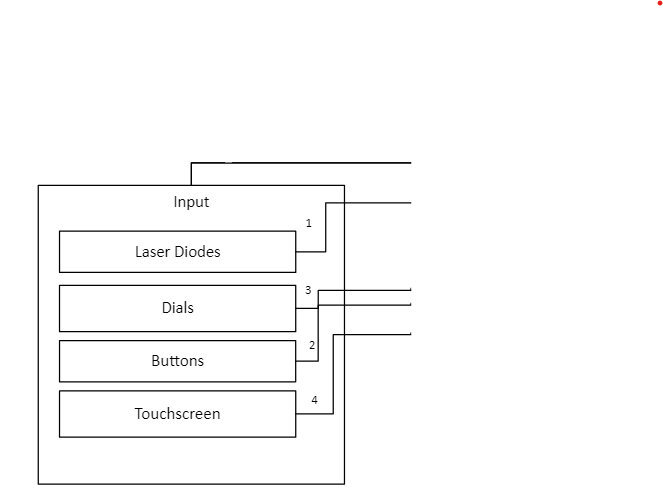
\includegraphics[width=0.60\textwidth]{images/InputSubsystem}
 \caption{Touchscreen}
\end{figure}

\subsubsection{Assumptions}
The touchscreen should be used as the primary way to interact with the control unit


\subsubsection{Responsibilities}
The touch screen main responsibility is to function as a visual output and as a way to interact with the OS and program which will have the user settings and sound settings


\subsubsection{Subsystem Interfaces}

\begin {table}[H]
\caption {Subsystem interfaces} 
\begin{center}
    \begin{tabular}{|  p{1cm}  |p{6cm}  |p{3cm}  |p{3cm} |}
    \hline
    ID & Description & Inputs & Outputs \\ \hline
    \#1& Takes input from the user by pressing on the screen also displays visuals& User input& \pbox{3cm}{UserSettings}\pbox{3cm}{Sound Settings}\\\hline
    \end{tabular}
\end{center}
\end{table}

